\documentclass{article}
\usepackage{graphicx}
\usepackage{hyperref}
\usepackage{listings}
\usepackage{xcolor}
\usepackage{tikzsymbols}
\usepackage{float}

\lstset{
    basicstyle=\ttfamily,
    backgroundcolor=\color{gray!30},
}

\title{Active Directory}
\begin{document}
\maketitle

\graphicspath{ {./Images/} }
\tableofcontents

\section{Introduction}
It took me far too long to realize the significance of the word "Directory" in Active Directory. So that never happens, again, here is Mr. Bing:

\textbf{Active Directory} (AD) is a directory service developed by Microsoft for Windows domain networks. 
It is included in most Windows Server operating systems as a set of processes and services. 
A directory, in the context of AD, is a hierarchical structure that stores information about objects on the network.
A directory service, such as Active Directory Domain Services (AD DS), provides the methods for storing directory data and making this data available 
to network users and administrators.

AD is both a database and a set of services that connect users with the network resources they need to get their work done. 
The database (or directory) contains critical information about your environment, including what users and computers there are and who’s allowed to do what. 
AD DS is a distributed database that stores and manages information about network resources as well as application-specific data from directory-enabled applications. 
The Active directory database uses the “Extensible Storage Engine (ESE)” which is an indexed and sequential access method (ISAM) database.

\textbf{LDAP} (Lightweight Directory Access Protocol) is an application protocol for working with various directory services. 
Directory services, such as Active Directory, store user and account information, and security information like passwords. 
The service then allows the information to be shared with other devices on the network. LDAP orchestrates searching in Active Directory. 
When a user searches for a user, computer, or printer, LDAP runs a search and finds the results. Based on multiple levels of permissions on Active Directory, 
users get access to information and resources through LDAP authentication. LDAP administrators require elevated permissions to add or manipulate information in 
your AD repository database.

\section{Domain Controller Deployment}
This step is very easy but Chris said I had to document it. 
Go to the add roles and features wizard, server roles, and check
"Active Directory Domain Services." After it finishes downloading,
click the yellow warning icon in the top right of the Server Manager.
The yellow icon says "Post Deployment Configuration".

\subsection{Making a new forest}
In the Deployment Configuration, select "Add a few forest".

In the text field that says "Root domain name", you will put the Fully
Qualified Domain Name (FQDN).

\paragraph{FQDN guidelines:}

\begin{enumerate}
\item \textbf{Naming}:
\begin{itemize}
        \item Use a subdomain of a domain you own, e.g., \texttt{ad.example.com}.
        \item Avoid using the exact public domain name.
\end{itemize}

\item \textbf{Length and Characters}:
\begin{itemize}
        \item FQDN should be 155 characters or fewer.
        \item Use letters (A-Z, a-z), numbers (0-9), and hyphens. No special characters.
\end{itemize}

\item \textbf{Uniqueness}:
\begin{itemize}
        \item Ensure no conflicts with existing names on your network.
\end{itemize}

\item \textbf{NetBIOS Name}:
\begin{itemize}
    \item The NetBIOS name is a legacy computer name format, typically shorter and without domain suffixes.
    \item For AD DS, it's a non-FQDN version of your domain name, often the prefix of your FQDN. Example: For \texttt{corp.example.com}, the NetBIOS name could be \texttt{CORP}.
    \item It's used for backward compatibility with older systems and applications that don't recognize FQDNs.
    \item Ensure it's unique within your network to prevent conflicts.
\end{itemize}

\item \textbf{Avoid}:
\begin{itemize}
        \item Names like \texttt{www}, \texttt{public}, \texttt{com}, \texttt{net}, \texttt{org}.
\end{itemize}
\end{enumerate}

After the domain is created, the built-in local "Administrator" 
account of the server becomes the domain "Administrator" 
account for that domain.

\paragraph{Directory Services Restore Mode}
A special boot mode for Windows Domain Controllers used for repairing, 
restoring, or analyzing Active Directory. In the event of a compromise 
or corruption of the domain controller, DSRM provides an isolated 
environment to restore from backups, conduct forensic analysis, or 
manually rectify issues. It's essential for maintaining the integrity 
and security of Active Directory services.

\subsection{Adding to an existing forest}
When adding a new Domain Controller to an existing forest, you should first join the machine to the domain.
The two machines must have different SIDs. Use the SIDCHGL program as described in the deployment section. 

\section{Network}
To edit your network settings, follow these directions:

Control Panel $\rightarrow$ Network and Sharing Center $\rightarrow$
Change Adapter Settings $\rightarrow$ Click "Internet Protocol Version 4 (TCP/IPv4)

\begin{figure}[]
        \centering
        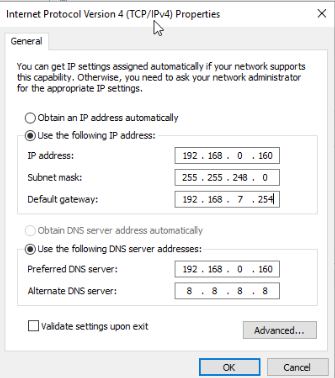
\includegraphics[width=1\textwidth]{SampleDCIPv4.png}
        \caption{Example IPv4 Settings}
        \label{fig:IPv4Settings}
\end{figure}

We have two goals in this menu: setting a static IP (to whatever) and setting the DNS servers. 
On non domain controllers, the DNS should be set to use DC1 and DC2.
On the domain controllers, the DNS should be set to use the other domain controller and the internet (e.g. 8.8.8.8 for Google's DNS).

\subsection{Setting a Static IP}
For an image, see Figure~\ref{fig:IPv4Settings}

You can set the static IP to any IP not currently in use.
(Maybe you can kick machines off of their IP, but that is probably not advised.)
Once you have picked your IP, put it in the \textbf{IP Address} field.
I am not sure how to determine the subnet mask manually, so I run \textbf{ipconfig} in powershell
and use the subnet mask it gives.
To determine the default gateway, you can run \textbf{ipconfig} or \textbf{route print}.
It is also possible to find the default gateway by running \textbf{ip route show} in the Proxmox console. 


\subsubsection{Setting the DNS Servers}
For an image, see Figure~\ref{fig:IPv4Settings}

I assume you have 2 Domain Controllers.

The Domain Controllers should have their DNS set to
\begin{enumerate}
        \item IP of the other Domain Controller
        \item Own IP (aka the static IP you set)
        \item Some other DNS that can go on the internet, i.e. 1.1.1.1 or 8.8.8.8
\end{enumerate}

To set more than 2 DNS servers, go to "Advanced" and then the DNS tab.

This step is less complicated than the last step. However, you can Red-Team yourself (I speak from experience...), so be careful.

On non domain controllers, both DNS servers should point to the domain controllers.

\textbf{Do not worry if you disconnect after doing this!!!}
The IP address of the server has changed, of course your rdp connection to it will be cut.

\section{Useful Videos}
This is a list of useful videos for understanding active directory.
At some point I should watch all of the videos, take notes on them, and put them in the document.
\begin{enumerate}
        \item \href{https://youtu.be/n5suPvKqo_Y}{FSMO Roles} (not very good but idk what FSMO role are and it is important)
        \item \href{https://youtu.be/5rEA7vRV3VE}{Professor Messer LDAP/LDAPS}
        \item \href{https://youtu.be/2w1cesS7pGY}{Sean Metcalf Active Directory Overview}
        \item \href{https://youtu.be/ze1UcSLOypw}{Sean Metcalf Active Directory Attacks}
        \item \href{https://youtu.be/Lz6haohGAMc}{More Sean Metcalf Active Directory}
        \item\href{https://youtu.be/b6GUXerE9Ac}{Even more Sean Metcalf Active Directory}
\end{enumerate}

\section{Enabling LDAPS}
Run the command certutil -verifystore MY

\section{Why do forests exist?}
\subsection{What is a forest}
A forest is a collection of one or more domains that 
share a common schema, configuration, and global 
catalog. The forest represents the highest 
level of logical container in Active Directory.

Trusts can be manually configured between different forests if required.

Certain forest-wide data, like the schema, 
is replicated to all domain controllers in all domains within the forest.

They can be used for replication and for
easier management across multiple geographic regions.

\subsection{What is a domain}
"A domain represents a database. 
That database holds records about
 network services-things like computers, users, groups and other 
 things that use, support, or exist on a network. The domain database is, 
 in effect, Active Directory."
 - Robert R. King

A domain is associated with a single DNS namespace (e.g., example.com).

By default, all domains within a forest have two-way, 
transitive trusts, meaning resources can be easily 
shared across domains in the same forest.

\subsection{What is a schema?}
\textbf{Active Directory Schema:}
\begin{itemize}
  \item Serves as the blueprint for permissible objects and attributes within Microsoft's Active Directory (AD).
\end{itemize}

\textbf{Key Elements:}
\begin{itemize}
  \item \textit{Object Classes:} Define permissible objects like users, groups, and computers.
  \item \textit{Attributes:} Specify properties an object can have, e.g., first name, last name for a user.
  \item \textit{Syntax:} Dictates the type of data an attribute can contain.
  \item \textit{Constraints:} Apply rules or limitations on attributes, such as mandatoriness.
  \item \textit{Object Identifiers (OIDs):} Ensure global uniqueness for object classes and attributes.
\end{itemize}

\textbf{Importance of Schema:}
\begin{itemize}
  \item \textit{Standardization:} Enforces consistent creation and management of objects.
  \item \textit{Extensibility:} Allows for custom object classes and attributes.
  \item \textit{Search Optimization:} Enables efficient querying via well-designed indexing.
  \item \textit{Security:} Restricted to administrators with special permissions.
  \item \textit{Interoperability:} Facilitates uniform interpretation of object data by various applications.
\end{itemize}

\textbf{Schema Modification:}
\begin{itemize}
  \item Sensitive, forest-wide operation requiring careful planning, testing, and coordination.
\end{itemize}


\subsection{Historical limits of domains}
In old versions of AD, a single domain could handle up to around 
10 million objects. However, these were not strict limits 
and more of an operational guideline. 

For Active Directory Domain Services in Windows Server 2008 and later, 
Microsoft stated that the maximum supported number of objects 
in Active Directory is 2.15 billion objects. 

There is a limit of $2^{30} \approx 10^9$ billion security 
identifiers (SIDs) over the life of a domain 
due to the size of the global relative identifier (RID) 
pool of 30 bits that makes each SID 
(that is assigned to user, group, and computer accounts) in a domain unique
\end{document}